%%%%%%%%%%%%%%%%%%%%%%%%%%%%%%%%%%%%%%%%%%
%                                        %
% Luther Michaels                        % 
% ECE 351-52                             %
% Lab 7                                  %
% October 21, 2021                       %
% Block Diagrams and System Stability    %
%                          Lab Report    %
%                                        %
%%%%%%%%%%%%%%%%%%%%%%%%%%%%%%%%%%%%%%%%%%

%%%%%%%%%%%%%%%%%%%%%%%%%%%%%%%%%%%%%%%%%%%
%%% DOCUMENT PREAMBLE %%%
\documentclass[12pt]{report}
\usepackage[english]{babel}
\usepackage{url}
\usepackage[utf8x]{inputenc}
\usepackage{amsmath}
\usepackage{graphicx}
\graphicspath{{images/}}
\usepackage{parskip}
\usepackage{fancyhdr}
\usepackage{vmargin}
\usepackage{listings}
\usepackage{hyperref}
\usepackage{xcolor}

\definecolor{codegreen}{rgb}{0,0.6,0}
\definecolor{codegray}{rgb}{0.5,0.5,0.5}
\definecolor{codeblue}{rgb}{0,0,0.95}
\definecolor{backcolour}{rgb}{0.95,0.95,0.92}

\lstdefinestyle{mystyle}{
	backgroundcolor=\color{backcolour},   
	commentstyle=\color{codegreen},
	keywordstyle=\color{codeblue},
	numberstyle=\tiny\color{codegray},
	stringstyle=\color{codegreen},
	basicstyle=\ttfamily\footnotesize,
	breakatwhitespace=false,         
	breaklines=true,                 
	captionpos=b,                    
	keepspaces=true,                 
	numbers=left,                    
	numbersep=5pt,                  
	showspaces=false,                
	showstringspaces=false,
	showtabs=false,                  
	tabsize=2
}

\lstset{style=mystyle}

\setmarginsrb{3 cm}{2.5 cm}{3 cm}{2.5 cm}{1 cm}{1.5 cm}{1 cm}{1.5 cm}

\title{7}	% Title						
\author{Luther Michaels}	% Author		
\date{October 21, 2021}   % Date

\makeatletter
\let\thetitle\@title
\let\theauthor\@author
\let\thedate\@date
\makeatother

\pagestyle{fancy}
\fancyhf{}
\rhead{\theauthor}
\lhead{\thetitle}
\cfoot{\thepage}
%%%%%%%%%%%%%%%%%%%%%%%%%%%%%%%%%%%%%%%%%%%%

\begin{document}
	
%%%%%%%%%%%%%%%%%%%%%%%%%%%%%%%%%%%%%%%%%%%%%%%%%%%%%%%%%%%%%%%%%%%%%%%%%%%%%%%%%%
%%% TITLE PAGE %%%
\begin{titlepage}
	\centering
	\vspace*{0.5 cm}
	
	\begin{center}    
		\textsc{\Large   ECE 351 - Section \#52}\\[2.0 cm]	
	\end{center}  
	\textsc{\Large Block Diagrams and System Stability }\\[0.5 cm]
	\rule{\linewidth}{0.2 mm} \\[0.4 cm]
	{ \huge \bfseries \thetitle}\\
	\rule{\linewidth}{0.2 mm} \\[1.5 cm]
	\begin{minipage}{0.4\textwidth}
		\begin{flushleft} \large
		\end{flushleft}
	\end{minipage}~
	\begin{minipage}{0.4\textwidth}
		\begin{flushright} \large
			\emph{Submitted By:} \\
			Luther Michaels \break
				
			\emph{Submission Date:} \\
			October 21, 2021
		\end{flushright}
	\end{minipage}\\[2 cm]
\end{titlepage}
	
%%%%%%%%%%%%%%%%%%%%%%%%%%%%%%%%%%%%%%%%%%%%%%%%%%%%%%%%%%%%%%%%%%%%%%%%%%%%%%%%%%
%%% TABLE OF CONTENTS %%%
	
\tableofcontents
\pagebreak
	
%%%%%%%%%%%%%%%%%%%%%%%%%%%%%%%%%%%%%%%%%%%%%%%%%%%%%%%%%%%%%%%%%%%%%%%%%%%%%%%%%%
%%% LAB REPORT %%%
\renewcommand{\thesection}{\arabic{section}}
\section{Introduction}

The main concept of this lab is that of Laplace-domain block diagrams. The goal is to introduce open-loop and closed-loop systems and build an understanding of both how to determine their transfer function from a block diagram and how to categorize their stability. Python commands will be used to derive the forms from which this inference may be made. \\

An open-loop system is a direct path from the input to the output, providing good performance and speed. A closed-loop system can include a feedback loop on its path and can thus respond to changes. A stable system is one which for all bounded inputs, the output is also bounded. Practically, if a system contains at least one pole that is not in the left half plane of the complex representation, it must be unstable. Several important functions for this lab procedure will be scipy.signal.convolve(), scipy.signal.residue(), scipy.signal.tf2zpk(), and scipy.signal.step(). We will come to see that the convolve function can be used to perform an expansion; scipy.signal.tf2zpk() can provide the zeros, poles, and gain of an input filter. All functions and plots can be produced using proper Python derivation and implementation written within the Spyder software. \\
	
\section{Equations}
	
\begin{align}
	G(s) &= \frac{s + 9}{(s^2 - 6s - 16)(s + 4)} \\
	&= \frac{-0.35}{s + 2} + \frac{0.208}{s + 4} + \frac{0.1417}{s - 8} \nonumber
\end{align}
\begin{align}
	A(s) &= \frac{s + 4}{s^2 + 4s + 3} \\
	&= \frac{1.5}{s + 1} - \frac{0.5}{s + 3} \nonumber
\end{align}
\begin{align}
	B(s) &= s^2 + 26s + 168 \\
	&= (s + 12)(s + 14) \nonumber
\end{align}
\begin{align}
	H_o(s) &= G(s)A(s) \\
	&= \frac{-0.44}{s + 1} + \frac{0.7}{s + 2} - \frac{0.27}{s + 3} - \frac{4.93 \times 10^{-16}}{s + 4} + \frac{0.0172}{s - 8} \nonumber
\end{align}
\begin{align}
	H_c(s) &= \frac{G(s)A(s)}{1 + G(s)B(s)} \\
	&= \frac{(numG)(numA)}{denA(denG + (numG)(B))} \\
	&= \frac{s^2 + 13s + 36}{2s^5 + 41s^4 + 500s^3 + 2995s^2 + 6878s + 4344} \nonumber
\end{align} \\

\section{Methodology}

As prescribed in the lab manual, the first task of Part 1 in this lab was to rewrite $ G(s) $, $ A(s) $, and $ B(s) $ in factored forms and identify their poles and zeros. This was facilitated by entering Equations 1 and 2 in Python using sets of numerator and denominator matrices. These two arrays were then input into the scipy.signal.residue() function to find the roots and poles. Finally, any zeros were identified by setting the initial numerators to zero. Before assigning the denominator of $ G(s) $ in Equation 1, the two factors were expanded using the scipy.signal.convolve() function. The zeros and poles of $ B(s) $ in Equation 3 were found through hand-derived arithmetic factorization. \\

In Task 2 of Part 1, verification of the results in Task 1 was requested using the function scipy.signal.tf2zpk(). The numerator and denominator matrices for $ G(s) $ and $ A(s) $ were placed as the inputs to this function in turn, and the returned zeros, poles, and system gain were printed. $ B(s) $ was written as a single matrix containing the coefficients in Equation 3. The numpy.roots function was then provided this matrix, and the roots/zeros were printed. The resultant zeros and poles of each were then compared with the those obtained in the prior task. \\

Task 3 of Part 1 required that the open-loop transfer function of the block diagram shown in the manual be expressed in factored form. As the open-loop path does not include the feedback, the general equation was determined to be Equation 4. The two equations were substituted in, producing the expression below.

\begin{equation*}
	H_o(t)= \frac{(s + 9)(s + 4)}{(s^3 - 2s^2 - 40s - 64)(s^2 + 4s + 3)} \\
\end{equation*}

The expansion of the result's numerator and denominator were found using the scipy.signal.convolve() function and placed in individual matrices. These two matrices were input in the scipy.signal.residue() function in order to determine the roots and zeros, enabling the construction of the factored form. \\

The fourth task of Part 1 inquired whether the open-loop response was stable. This answer and its reasoning are provided in the Results section. \\

Task 5 of Part 1 wanted a plot of the step response for the open-loop transfer function. Given that scipy.signal.convolve() was already used in Task 3 to implement the numerator and denominator matrices, these matrices could be directly input into the scipy.signal.step() function along with the time variable.  After including a step size of $ 1\times 10^{-5} $ for good resolution and initializing the time interval with numpy.arange, the returned values of scipy.signal.step() were plotted, utilizing the commands in the matplotlib.pyplot to format and label the graph. As directed in Task 6, a comparison the results found in Tasks 4 and 5 is provided in the Results section.  \\

The first task of Part 2 requested the closed-loop transfer function of the block diagram be expressed in terms of the block functions' numerators and denominators. Given that the closed-loop path includes all block functions, the negative feedback loop could be simplified directly to derive Equation 5. The derivation to produce the required form shown in Equation 6 is provided below.

\begin{align*}
	H_c(s) &= \frac{Y(s)}{X(s)} = \frac{G(s)A(s)}{1 + G(s)B(s)} \\
	&= \frac{\frac{numG}{denG}\frac{numA}{denA}}{1 + \frac{numG}{denG}B} \\
	&= \frac{(numG)(numA)}{(denG)(denA)(1 + \frac{numG}{denG}B)} \\
	&= \frac{(numG)(numA)}{denA(denG + (numG)(B))} \\
\end{align*}

Task 2 of Part 2 was to find the expanded form of the closed-loop transfer function using scipy.signal.convolve() and scipy.signal.tf2zpk() as needed. Substituting the numerators and denominators into Equation 6, the equation below was produced.

\begin{equation*}
	H_c(s) = \frac{(s + 9)(s + 4)}{(s^2 + 4s + 3)((s^3 - 2s^2 - 40s - 64) + (s + 9)(s^2 + 26s + 168))}
\end{equation*}

The numerator was expanded using scipy.signal.convolve() as well as the two terms within the right factor of the denominator. After adding the latter resultant expansion terms with the second polynomial in the right factor, the total denominator expansion was found by combining the lower terms into scipy.signal.convolve(). The expanded form of the closed-loop transfer function was then written by printing the final numerator and denominator. \\

The third task of Part 2 questioned if the closed-loop response was stable. This answer and its reasoning are provided in the Results section. \\

Task 4 of Part 2 asked that the step response of the closed-loop transfer function be plotted. The final numerator and denominator matrices found in Task 2 of Part 2 were placed into the scipy.signal.step() function with the time variable. The two outputs of this function were then plotted, formatting the graph with the standard sequence of plotting instructions. As requested by Task 5, a comparison of the outcomes of Tasks 3 and 4 can be found in the Results section.\\

Github Link: \url{https://github.com/Luther-Michaels} \\
	
\section{Results}

As dictated by scipy.signal.residue(), the poles of $ G(s) $ were found as [$ -2 $, $ -4 $, $ 8 $] and of $ A(s) $ as [$ -1 $, $ -3 $]. The zeros of each function were isolated, finding $ G(s) $ with a zero at $ -9 $, $ A(s) $ at $ -4 $, and $ B(s) $ at $ -12 $ and $ -14 $. The derived factored forms of $ G(s) $, $ A(s) $, and $ B(s) $ are shown below. The poles shown in these results represent an equivalent form, as plugging a value for $ s $ into both the original and these factorizations yield the same results. Likewise, when plugging the zeros into the final expressions as $ s $, the results reach zero.

\begin{align*}
	G(s) &= \frac{s + 9}{(s^2 - 6s - 16)(s + 4)} = \frac{s + 9}{(s + 2)(s + 4)(s - 8)} \\
	&= \frac{-0.35}{s + 2} + \frac{0.208}{s + 4} + \frac{0.1417}{s - 8}
\end{align*}
\begin{align*}
	A(s) &= \frac{s + 4}{s^2 + 4s + 3} = \frac{s + 4}{(s + 1)(s + 3))} \\
	&= \frac{1.5}{s + 1} - \frac{0.5}{s + 3}
\end{align*}
\begin{align*}
	B(s) &= s^2 + 26s + 168 \\
	&= (s + 12)(s + 14)
\end{align*}

The printed results of the scipy.signal.tf2zpk() function for the second task are provided in the Appendix. Viewing the values of the zeros and poles, it is clear that they match those obtained in the prior result. This lends credence to both methods. \\

The factored form of the open-loop transfer function is shown below. The expanded form used in the Python derivation process is also provided to analyze the result. The validity of the factored form is supported by the fact that it incorporates the poles of both the functions it is built from. It has further been scrutinized by plugging a value for $ s $ into the original and expanded forms, concluding that all match and the result aligns with our expectation.

\begin{align*}
	H_o(s) &= \frac{Y(s)}{X(s)} = G(s)A(s) \\
	&= \frac{s^2 + 13s + 36}{s^5 + 2s^4 - 45s^3 - 230s^2 - 376s - 192} \\
	&= \frac{-0.44}{s + 1} + \frac{0.7}{s + 2} - \frac{0.27}{s + 3} - \frac{4.93 \times 10^{-16}}{s + 4} + \frac{0.0172}{s - 8}
\end{align*}
 
The expression for the open-loop transfer function found in the prior task indicates that the response will not be stable. This is because it includes a single pole ($ 8 $) that is not in left half plane of complex number representation. Consequently, the output will not stay bounded. One unstable pole makes the whole system unstable. \\

The following plot shows the step response of the open-loop transfer function. It is properly plotted over the time interval from 0 to 2s and displays good resolution. As with the poles of the function, the plot of the step response indicates an unstable system. This is shown by the right-hand exponential increase. The y-axis values make sense given the large coefficients of the negative terms in the denominator of the transfer function and indicate that the output is not bounded. In this way, the plot supports the hypothesis formed from the transfer function's poles. \\

\begin{center}
	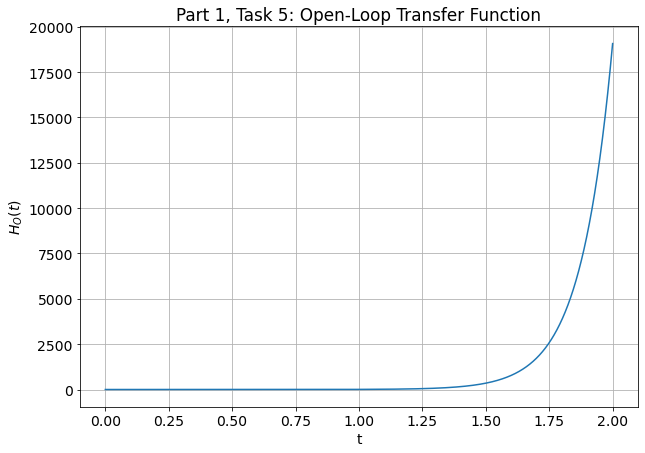
\includegraphics[scale = 0.6]{Lab 7 - Plots/Part1-Task5.png}\\[1.0 cm]
\end{center}

The equations below show the closed-loop transfer function expressed both in terms of the block functions' numerators and denominators and in its expanded form. By plugging the same value into $ s $ for the original closed-loop transfer function and the two forms, the validity of both can be shown. An important characteristic of the total resulting transfer function is that the denominator is comprised entirely of positive terms.

\begin{align*}
	H_c(s) &= \frac{Y(s)}{X(s)} = \frac{G(s)A(s)}{1 + G(s)B(s)} \\
	&= \frac{(numG)(numA)}{denA(denG + (numG)(B))} \\
	&= \frac{s^2 + 13s + 36}{2s^5 + 41s^4 + 500s^3 + 2995s^2 + 6878s + 4344}
\end{align*}

If the numerators and denominators are substituted into the result of Task 1 (Equation 6), it can be seen that the final denominator will only feature positive terms. This is likewise reflected in the expanded transfer function above. Because there are no negative terms, the factorization must be positive. The poles will then all be negative and thus in the left half plane. This means that the closed-loop response will be stable. \\ 

The plot below shows the step response of the closed-loop transfer function. The y-axis maximum over the same time interval is drastically smaller than that of the open-loop transfer function. This is because the function develops negative concavity as it extends right, and the output is consequently bounded. Given this fact, it is clear that the plot supports the conclusion inferred previously that the response will be stable. \\ 
	
\begin{center}
	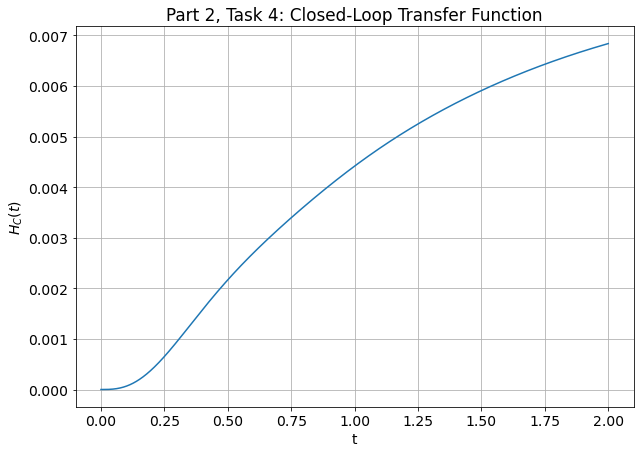
\includegraphics[scale = 0.6]{Lab 7 - Plots/Part2-Task4.png}\\[1.0 cm]
\end{center}
	
\section{Error Analysis}

I initially had difficulty in deriving the expanded form of the closed-loop transfer function. This was because I did not reduce the form utilizing the numerators and denominators before progressing. After simplifying the starting point, the Python commands became much simpler and the result was obtained. \\

\section{Questions}

1. Performing a convolution of factored terms using scipy.signal.convolve() in steps such as Part 1 Task 5 results in the expanded form because the default method is found through direct summation. The terms will be multiplied in order and then added together. This would not work with the user-defined convolution function from Lab 3 as the implementation alters the arrays containing its input. It tries to create extended arrays of equal length by appending zeros, but this shifts the order of magnitude that the input coefficients correspond to and changes the problem. \\

2. The difference between the open-loop and closed-loop systems starts with the fact that the open-loop does not include the negative feedback path.  In Part 1 and Part 2, it was identified that the open-loop system had unstable behavior, while the closed-loop system was stable. This is the direct result of their primary difference. Because the open-loop system goes straight from the input to the output, there is no possibility for determining changes through feedback. It has improved performance, but proves unstable without the adjustment. The closed-loop system, on the other hand, is stable due to its feedback. \\ 

3. The difference between scipy.signal.residue() used in Lab 6 and
scipy.signal.tf2zpk() used in this lab is in the information they return. While both provide the poles of their input, the former function returns the residue and coefficent of the direct polynomial term, while the latter gives the zeros and system gain. The scipy.signal.residue() function is more useful for general partial fraction expansion; scipy.signal.tf2zpk() is specifically applicable to filter analysis. \\

4. If we think of a system being stable as one that contains only poles in the left half plane of the complex representation, it is certainly possible for an open-loop system to be stable. Were the expressions for $ G(s) $ and $ A(s) $ to include only negative poles, the transfer function would have led to a stable system. Likewise, a closed-loop system could be unstable due to its feedback. If the feedback is influenced by a term that includes a positive pole, the response would be unstable. While one may tend towards stability over the other, each is still dependent on the block functions included in their paths towards the output. \\ 

5. The lab purpose and expectations were communicated clearly, but the deliverables were a little unclear/inconsistent in identifying the form of the final derivations that should be presented in Task 2 of Part 2. The total resulting transfer function is requested, but is not clear enough if this should be in factored or expanded form.

\section{Conclusion}

In this lab we were introduced to the concepts of open-loop and closed-loop circuits, practiced block diagram analysis, and furthered our understanding of system stability. It refined our skills in finding step response using scipy.signal.step() and partial fraction expansion using scipy.signal.residue(). It also presented the function scipy.signal.tf2zpk() for identifying zeros and poles, and showed that the function scipy.signal.convolve() could be used to find an expansion. It challenged us to combine multiple techniques into one derivation solution using Python. \\

If this lab were repeated, I would include a test of the Lab 3 convolution function meant to verify that the results do not match the expansion using the function scipy.signal.convolve(). This would help support the answer to one of the questions in the lab manual. I learned to better synthesize various approaches and solve problems analytically in this lab. Being able to see see the different steps and methodology needed to solve a problem will continue to be a useful skill in the future. \\

\newpage
\appendix
\section*{Appendix - Print Output}

Part 1, Task 2:
\begin{center}
	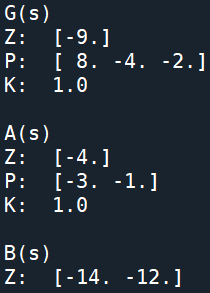
\includegraphics[scale = 1.25]{Lab 7 - Print Output/Part1-Task2.png}\\[1.0 cm]
\end{center}

\newpage
\begin{thebibliography}{111}
		
	\bibitem{S}
	Sullivan, Dennis M. (2018) {\it  Signals and Systems for Electrical Engineers I}. Nevada: CreateSpace Independent Publishing Platform.
		
\end{thebibliography}
\end{document}

% Lab Report based on template created by Roza Aceska.